\documentclass[a4paper,10pt]{article}

%\usepackage[utf8]{inputenc}
\usepackage{graphicx}
\usepackage{url}
\usepackage{float}
\usepackage{times}
\usepackage{multirow}
\usepackage{listings}
\usepackage{times}
\usepackage{paralist}
\usepackage{epsfig}
\usepackage{subfigure}
\usepackage[hypertex]{hyperref}
\usepackage{subfigure}
\usepackage{color}
\usepackage{ifpdf}

\newcommand{\I}[1]{\textit{#1}}
\newcommand{\B}[1]{\textbf{#1}}
\newcommand{\BI}[1]{\textbf{\textit{#1}}}
\newcommand{\T}[1]{\texttt{#1}}

\pdfpagewidth 8.5in
\pdfpageheight 11in 

\setlength\topmargin{0in}
\setlength\headheight{0in}
\setlength\headsep{0in}
\setlength\textheight{9in}
\setlength\textwidth{6.5in}
\setlength\oddsidemargin{0in}
\setlength\evensidemargin{0in}
\setlength\parindent{0.1in}
\setlength\parskip{0.25em}

\ifpdf
 \DeclareGraphicsExtensions{.pdf, .jpg}
\else
 \DeclareGraphicsExtensions{.eps, .ps}
\fi

\newcommand{\jha}[1]{ {\textcolor{red} { ***Jha: #1 }}}

\begin{document}
\title{\large Biomolecular Simulations and Distributed Computing on TG}

\author{Principal Investigaor: Shantenu Jha$^{1,2}$ \\ Co-Principal Investigaor: Joohyun Kim$^{1}$ \\ Co-Principal Investigaor: Yaakoub El Khamra$^{3}$\\\
   \small{\emph{$^{1}$Center for Computation \& Technology, Louisiana State University, Baton Rouge, 
USA}}
\\
  \small{\emph{$^{2}$Department of Computer Science, Louisiana State
      University, Baton Rouge, USA}}
\\
  \small{\emph{$^{3}$Texas Advanced Computing Center TACC, University of Texas, Austin, USA}}}



\date{10 July 2009}

\maketitle

\subsection*{Summary:} Over the past twelve to eighteen months, we have been involved in a wide 
range of computational science and computer science projects, requiring a range of simulations.
In this proposal we request 0.9M SUs for three distinct projects:
(i) understanding translocation of nucleic acid in $\alpha$-Hemolysin protein pores; (ii)
conformational switching of S-box riboswitch and, (iii) for developing and 
deploying distributed applications and the infrastructure required to facilitate
their development. 
The projects for which computer time is being requested are all funded projects -- some at the national level, and some
by local resources; those that are not funded by NSF/NIH form the basis for upcoming significant
NSF/NIH proposals. 
Additionally, the request for 0.9M SUs in this proposal 
is based upon the projected science problems as outlined below as well as a proven
track record of
{\it successfully} utilising approximately 350,000SUs in the last 9-10 months (in increments
of several and concurrent 50,000 chunks).

\subsection*{Project 1: Nucleic Acid Translocation through Alpha-Hemolysic Protein Nanopore}

Translocation of nucleic acid strands through confined protein pores has biological relevance in instances 
such as viral transfer of genetic material across a membrane.
Nanopore current recording experiments can reveal information on a polymer translocating through a pore 
such as the well characterised protein pore $\alpha$-Hemolysin (Fig.1). A nanopore is inserted into a lipid 
bilayer and a transmembrane potential is applied. The ionic current through the pore is measured and the 
translocation of polymers through the pore causes a measurable current blockade by obstructing the flow 
of electrolytes through the pore.
With high enough output resolution, the sequence of a DNA strand could be attained. By simulating the 
translocation event, our understanding of the microscopic processes involved will increase. This could 
move the field towards genetic sequencing.

The high-level scientific objective for this project is to compute the free energy
profile of the translocation process of DNA along the vertical axis of a a
transmembrane protein pore buried in a lipid membrane bilayer. This is a project that has been ongoing for nearly two years (which was 
initiated before my transition to LSU),  has consumed a total of $\approx$ 1.5M SUs
so far (of which 200,000 are on LONI) and we are now very close to 
major publication in a high-profile journal (Fall 2008). 
Over the past 24 months, we have been performing an extensive series of
simulations of DNA translocation through the $\alpha$-hemolysin nanopore by a
novel combination of algorithm and computational infrastructure. The possible
parameter space of the problem that needs to be explored is huge, but through
our studies we have
determined the optimal values at which to perform the non-equilibrium simulations.
%simulations. This work follows as a natural extension of the work done as part
%of the SPICE project which won the HPC Analytics Challenge Award at
%SuperComputing'05 and the Life Science Award at International Supercomputing
%Conference 2006. 
The project uses the parallel MD code NAMD and as also led to a 
grid-enabled version of NAMD developed by us to perform steered MD simulations
including the capability to connect to distributed haptic devices. This work is currently 
funded by the UK's EPSRC (equivalent to the US NSF).
Current and near-future
work, also forms the basis of a joint US-UK submission to the NSF (in collaboration 
with Prof.'s Zuzanna Siwy (UC-Irvine) and Stefan Howorka (London)). 

{\bf Principal scientific objectives:} To compute the free
energy profile of the translocation process of DNA along the vertical axis of
a transmembrane protein pore buried in a lipid membrane bilayer.  There are
presently established methods of experimentally deducing the base sequence of
nucleic acid chains, however, such methods are not economically accessible
enough to allow for the decoding of DNA for purposes such as in medical
analysis. As Akeson~\cite{akeson} have shown, threading nucleic acid chains through
transmembrane porous proteins (such as $\alpha$-hemolysin) in a single channel
current recording apparatus can provide information indicating sequence. At
the resolution of the data retrieved from the experiments of Akeson,
conclusions were limited, not allowing the differentiation of individual
bases. It is proposed that steps towards individual base coding by this method
can be made by increasing the translocation time of nucleic acid chains
through the pore, or making the extent of blockage more distinct based on the
type of base. This can be achieved either by chemical modification of the pore
surface or modification of the nucleic acid chain itself, yielding a higher
resolution current readout. Experimentally, Akeson showed that threading
single-stranded dA and dC based nucleic acid chains results in different
translocation times and different degrees of pore blocking. To understand
experimental results and explore alterations to this method, computer
simulations can be performed that compute the free energy profile of the
various ssDNA sequences that translocate and thus provide the required insight
into the physical mechanisms responsible for the significant change in the
translocation time. Using NAMD our simulations  mimic - in a 'natural'
environment - the translocation process. 

We use constant velocity Steered Molecular Dynamics (cv-SMD) is used to reduce simulation computation to practical levels. In cv-SMD, fast translocation is performed by pulling the front most residue of a single stranded DNA strand at constant velocity.  The equilibrium free energy profile is extracted from the non-equilibrium work done using Jarzynski�s Equality~\cite{jarz}.
In addition to verifying the experimental results (which should be amenable to
relatively small scale simulations), moving 20-base long single-stranded A and
dC nucleic acid chains inside the protein pore and analysing differences in
the free energy profile/work done in the process, will test the ability of our
method to distinguish difference sequences.
The ability to compute via simulations, the 
free energy profiles along sub-sections of the pore has immediate consequences for
DNA sequencing.

%Following that we would also
%like to simulate the movements of longer chains of 50-base length (of both dA
%and dC) in order to explore the effect that the length of the DNA strand has
%on the profile(s).

\begin{figure}
\begin{center}
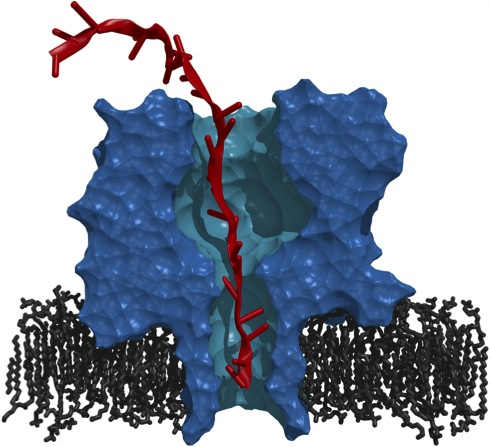
\includegraphics[scale=0.5]{pore_dna-1.jpg}
\end{center}
\caption{Single stranded DNA translocation through $\alpha$-Hemolysin. A cross-section of the protein 
pore $\alpha$-Hemolysin is depicted in blue. Red represents a single strand of DNA (3 end at the bottom).  
Black represents the lipid bilayer.  The DNA strand is translocted from the cis (top) entrance to the trans 
(bottom) entrance.}
\label{}
\end{figure}

\begin{figure}
  \subfigure[]{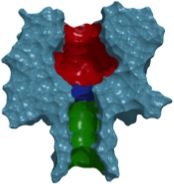
\includegraphics[scale=0.750]{pore_structure-1}}  \hspace{1.5in}
  \subfigure[]{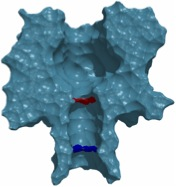
\includegraphics[scale=0.750]{pore_structure-2}}
\caption{These simulations are concerned with translocation at the constriction (blue) and beta barrel 
(green) of $\alpha$-HL. Red represents the alpha chamber.
Here the translocation resistance is highest due to the pore dimensions.
Key pore residues present themselves when pulling poly-Adenine across this region at 0.004 A/ps. 
Methionine residue 113 (red) and Leucine residue 135 (blue) show peaks in work profile.}
 \label{model}
\end{figure}

\begin{figure}
  \subfigure[]{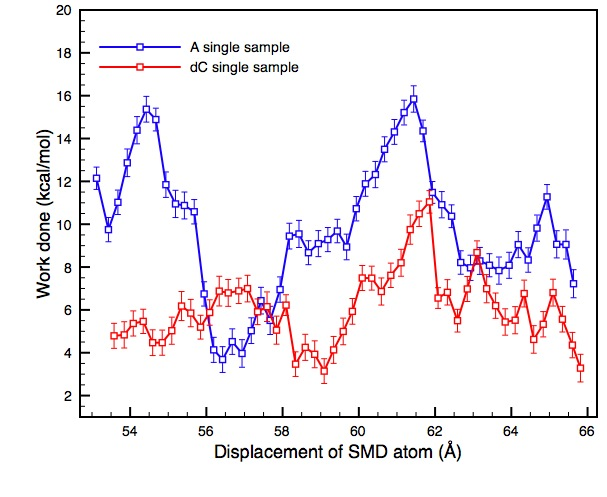
\includegraphics[scale=0.4]{single_sample_A_vs_dC_135}}  
  \subfigure[]{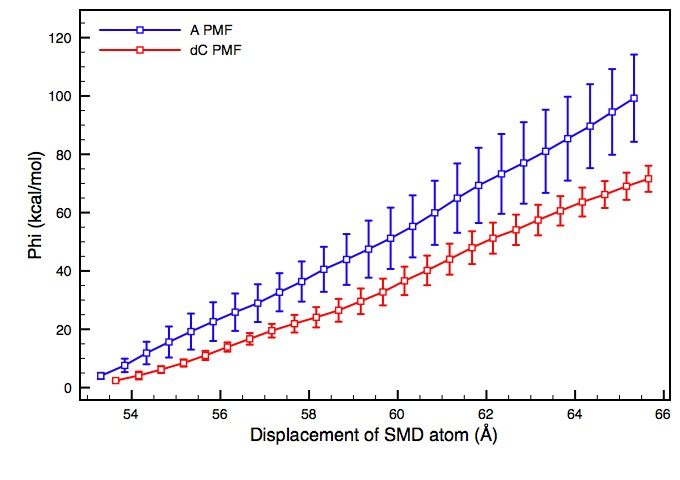
\includegraphics[scale=0.4]{dC_vs_A_PMF}}
\caption{Simulation results show the difference in the work profile of translocation between nucleotide
chains with differing secondary structure (A vs dC). The figure to the left is for a single sample -- local
energetic profiles, which is capable of distinguishing the main features and events contributing to the profile.
The figure to the left is the total work profile over the complete pore, averaged over several samples (six in 
this case). There are indications that the total translocation work energy distinction between A and dC lies 
well beyond the error bars.}
 \label{model}
\end{figure}



\begin{figure}
\begin{center}
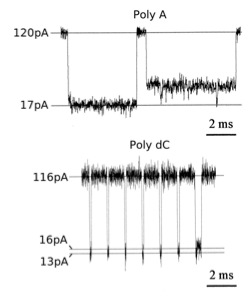
\includegraphics[scale=0.60]{polyA_polydC.jpg}
\end{center}
\caption{Single molecule current traces for poly Adenine and poly-deoxy-Cytosine2.
Poly-A takes ~20 times longer to translocate than poly-dC.
; experimental evidence of different translocation times for oligo-nucleotide chains
of A and dC (differing in secondary structure); the precise mechanism of this
difference is not understood by experiments; our computer simulations provide
inside in to the different "dwell" times.}
\label{}
\end{figure}


{\bf Resources Requested:}

The code we use is NAMD - a well established, community code that has been
extensively validated and tested for scalability (for more
benchmark/performance data, see:
http://www.ks.uiuc.edu/Research/namd/performance.html). Timings for our system
(approximately 320,000 atoms) as benchmarked are: \\
%1.30 days/ns on 64 cores, 0.60 days/ns on 128 cores, 0.35 days/ns on 256 cores.
Back when queen bee was running slower~\footnote{we helped diagnose
a hardware problem with Queen Bee} and we were using 384 processors: \\ % \newline
  \indent performance on 384 CPUs 0.0529952 s/step (0.306685 days/ns) \newline
Now it's faster and we are using 256 processors the performance is: \newline
  \indent on 256 CPUs : 0.0506383 s/step (0.293045 days/ns)  \footnote{with similar performance on Tezpur}

Thus, simulations of our systems are most efficient on 256 cores (consistent with the NAMD rule-of-thumb of approximately 1000 atoms per core), and it
takes approximately 2000 CPU hrs to simulate one nanosecond. 
Thus, at a optimal pulling speed, (as there is a compromise between statistical and systematic errors),  it takes the equivalent of $\approx$ 5ns of simulation time for the ssDNA to be pulled through the relevant and interesting portion of the pore. Given that these are non-equilibrium
simulations, based upon our experience from the SPICE project~\footnote{see http://www.realitygrid.org/Spice and publications therein}, we need 
on average 8-12 simulations to get a measure of the free energy profile.  Taking
10 as the typical number of samples required, we need 10 x 5 x 2000 = 100000 CPU hrs, to
gather enough statistics for a single  translocation study (for example, a
specific nucleotide sequence and length).
A single translocation study represents just the beginning of many simulations that will be needed to explore
the (rich) phase-space of this problem in order to understand the physical
properties of this important system and the specific science problems.
Specifically, the science problems that we are addressing are:
\begin{itemize}
\item Effect of secondary structure on the translocation times
\item  Exploring specific interactions that are the dominant component
of the "dwell" time within the pore
\item Understanding the difference between the translocation properties
of a single nucleotide versus a 20-mer oligo-nucleotide, so as to 
be able to discern the "single" compoent in the "extended, collective"
dynamics of longer polymer chains
\item Mutation studies need to be performed to help distinguish steric interactions from other (e.g.,
hydrophobic) interactions
\end{itemize}

The fundamental computational challenge arises from the requirement to perform
a multiple number (between 8-12) of samples of the same "pulling event"; this is
a consequence of the non-equilibrium simulations/methods and thus the stochastic nature of the simulations. However, in spite of this, the method used 
is still at least an order of magnitude quicker than "slow motion" real dynamics MD simulations.

We anticipate being able to make progress on items 1 (and related to it item 2)
and item 5; this is what we anticipate we will be able to achieve over the next six months. 
For each item, we anticipate a lower bound of 200,000 SUs; thus we are requesting
400,000 SU hours for project I. We will be back 
with a request for more hours if we were to effectively study the different specific
science objectives.


\subsection*{Project 2: Computational Study of non-coding Functional RNAs: Binding mechanism of Riboswitches}

%Increasing attention has focused on targeting RNAs for drug design~\cite{foloppe}. 

With increasing evidences indicating a critical role of nc-RNAs in transcriptional regulation and
translational regulation, increasing attention has focused on the potential of targeting RNA for drug
design~\cite{foloppe}.
However, because 
RNAs are flexible and highly negatively charged, many unresolved details on how RNA folds and binds with a small molecule/Proteins/RNAs remains to be understood.  With Riboswitches, there are interesting puzzles about how small molecules 
interact with RNAs and the coupling of those interactions with the conformational change of RNAs. 
Therefore, understanding the physico-chemical interactions between RNAs and small molecules and
the mechanisms through which small molecules trigger the conformational dynamics of RNA should 
provide the scientific basis for rational design of chemical compounds that target RNA.

\begin{figure}
  \subfigure[]{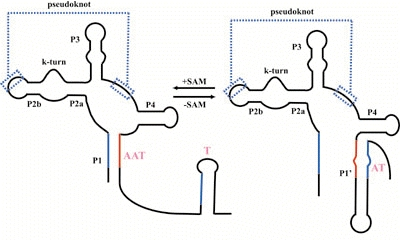
\includegraphics[scale=0.60]{ss-schema}} \hspace{0.05in}
  \subfigure[]{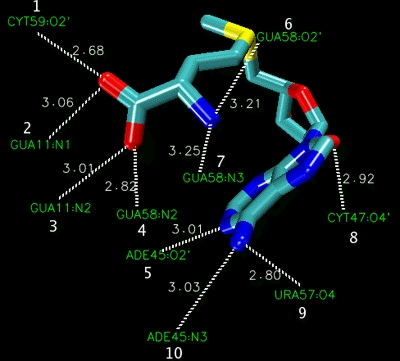
\includegraphics[scale=0.40]{ligand-atom2}}
\caption{Schematic of the secondary structures of s-box riboswitch with SAM bound (left; in the AAT state) and without SAM 
(right; in the AT state); predicted ligand-SAM interactions with s-box}
\end{figure}


\begin{figure}
  \subfigure[]{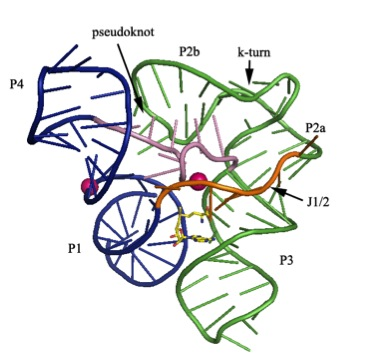
\includegraphics[scale=0.4]{sbox_3D}}
  \subfigure[]{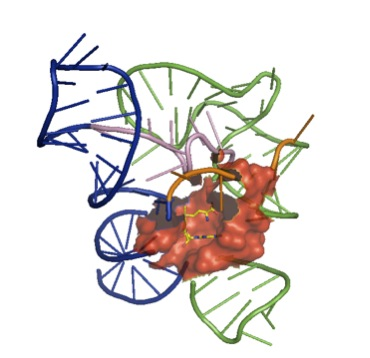
\includegraphics[scale=0.40]{binding_pocket-2}}
  \subfigure[]{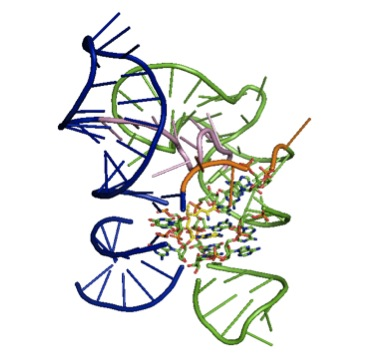
\includegraphics[scale=0.4]{binding_pocket-1}}
\caption{(i) The structure of the S-box riboswitch; (ii) S-box with SAM bound; (iii) Residue number: 7, 11, 
12, 45-47, 57-59, 88, 89}
\end{figure}


Riboswitches are regulatory RNAs that control the expression of downstream genes. Small metabolite 
molecules, such as amino acids, nucleotides, coenzymes etc., can bind to riboswitches as effectors in  vivo~\cite{mandal}. 
The S-box riboswitch (also called SAM-I riboswitch) is one member of the riboswitch family that
regulates the metabolism of sulfur and methionine. 
When S-adenosylmethionine (SAM) is absent, the
s-box occupies a more energetically favorable anti-terminator (AT) conformation. SAM can
specifically bind to the s-box inducing the formation of anti-anti-terminator (AAT) conformation,
which turns off the downstream genes by forming the terminator (T) (Figure 5a).
The S-box riboswitch can control the expression of biosynthetic proteins involved in sulfur metabolism 
through conformational change upon the binding of S-adenosylmethione (SAM)~\cite{brooke}. Although the 
structure of the s-box in the anti-anti-terminator (AAT) conformation has been solved via X-ray 
crystallography, it is just a static view of how SAM binds to the s-box. The goal of this study is to probe 
the dynamic interactions between the s-box riboswitch and SAM at the nanoscale and to explore 
determinants for the specificity. In addition, this study aims to understand the mechanism through which 
SAM perturbs the conformational equilibrium within the mRNA towards the AAT conformation.

\subsubsection*{Methods}

The starting point of all simulations is the X-ray crystal structure of SAM binding to the AAT conformation 
of s-box riboswith (PDB: 2GIS)~\cite{montange}. In the simulation of the SAM free s-box riboswitch, SAM 
is directly removed from the x-ray crystal structure and replaced with solvent water. The amber99bsc0
correction force field is used here~\cite{alberto}. Parameters for SAM are from the Generalized Amber 
Force Field (GAFF) and missing parameters are calculated using ANTECHAMBER~\cite{wang}. Positions 
of added hydrogens are guessed using PSFGEN within NAMD 2.6. Then the RNA molecules are solvated 
in a cubic solvent box of TIP3P waters with a 16A padding in all directions. Sodium and magnesium ions 
are randomly distributed at least 5 A away from the RNA molecules in order to neutralize charge of the 
system. The total number of atoms in the system is 56,000. Energy minimizations are carried out on all of the systems to remove bad contacts. Starting from 
0 K, the temperature is raised 10 K for every 10,000 steps and is held constant after reaching the desired 
temperature (310 K) using temperature reassignment. MD simulations are performed in the NPT ensemble 
with the pressure maintained using the Langevin piston method with a period of 100 fs and decay times of 
50 fs. The time step is 2fs for both equilibration and production phase. Bond lengths between hydrogens 
and heavy atoms are constrained using SHAKE. The long-range electrostatics is treated with the Particle 
Mesh Ewald (PME) method with a cutoff distance 12A.  VMD, wordom~\cite{moe} and homemade scripts are employed to analyze the trajectories. All snapshots 
of structural images are made using VMD.

%All simulations are performed using NAMD 2.6 on LSU (Tezpur) and LONI (Queenbee) Linux clusters. 


\subsubsection*{Initial Results}

\begin{figure}
   \subfigure[]{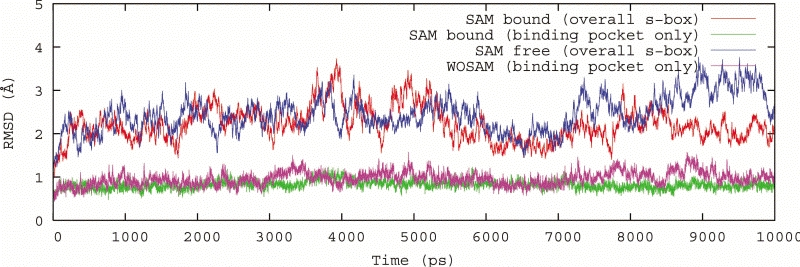
\includegraphics[scale=0.56]{rmsd}} \newline
   \subfigure[]{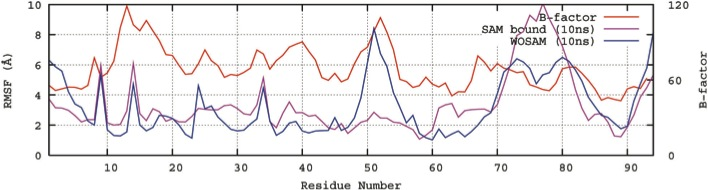
\includegraphics[scale=0.660]{RMSD_residue}}
\caption{RMSD of overall s-box and binding pocket only in SAM bound and WOSAM (short for the 
trajectory of SAM free s-box riboswitch) trajectories  with reference to the crystal structure; (b) Root mean square fluctation (RMSF) and B-factor of each residue of s-box riboswitch from MD trajectories}
\end{figure}

\begin{figure}
   \subfigure[]{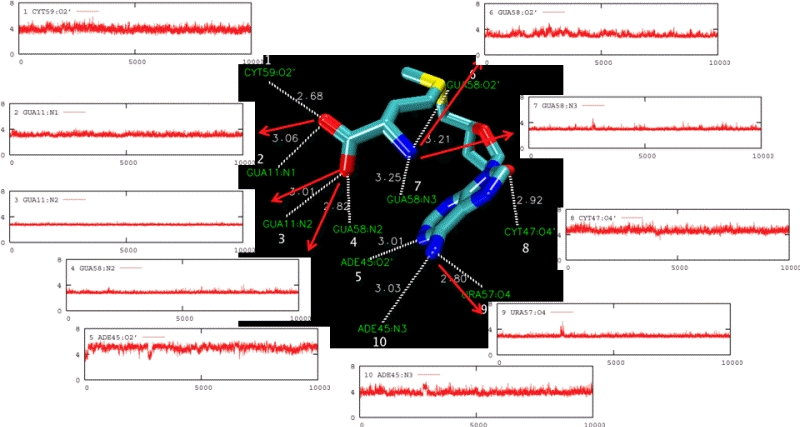
\includegraphics[scale=0.50]{distance}}
\caption{The time evolution plots of distance for SAM and S-box binding pocket
contacts for 10ns simulation. [x axis: time step (ps), y axis: distance (A)]}
\end{figure}

Related experiments and this work is carried out in collaboration with Prof. Fareed Aboul-ela. We are co-supervising Wei Huang, a second year Biology PhD student.
On the one hand, Molecular Dynamics (MD) simulations are employed to probe the interactions between SAM 
and the s-box riboswitch and examine the dynamics of the s-box riboswitch at the nanoscale. A 
significant  
advantage of these simulation is the ability to be able to explore details that are typically inaccessible to experiments; while at the same time providing the opportunity for  
our simulation results will be validated using biochemical and biophysical experiments. Therefore, the 
combination of simulation and experiment is a distinct feature of our project.
Our preliminary result suggests that the presence of SAM in the binding pocket reduces motions in the  sub-nanosecond time regime (Figure 7). Besides, five out of six stable contacts (red arrows) 
between SAM and the binding pocket are related to the methionine chain of SAM (Figure 8). 
This result demonstrates that the methionine chain is the critical component for SAM to be recognized by 
the s-box from other metabolite analogs. This result is consistent with results from the biochemical study 
of the binding of SAM and analogs of SAM to the s-box. 

MM-PBSA (Molecular Mechanics - Poisson Boltzmann Surface Area) is chosen to estimate the total binding free energy in term of distinct contributions with explicit physical
meaning.
The MM-PBSA method should help us understand the balance of different components and how
they are correlated with molecular recognition. In addition, PCA (Principle Component Analysis), cluster
algorithems and other applied mathematical algorithms has been applied to analyze MD trajectories.
In order to understand the conformational changes and the major dynamical
modes will require simulations to be to be extended to longer timescale, possibly into hundreds of 
nanoseconds (we are already touching the limit of 100ns!).
Specifically we will use the the long-time simulation to explore:

\begin{itemize}
\item To find out the collective motion difference between SAM bound and WOSAM, for SAM bound, there 
may be some collective motion among the binding pocket residues; WOSAM, how the collective motion 
changes?
\item Correlation of binding free energy with conformation clusters/PCA analysis
\end{itemize}

\begin{figure}
   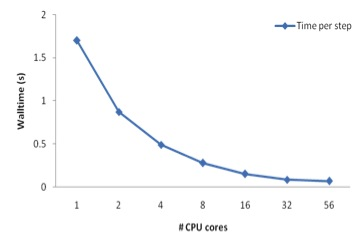
\includegraphics[scale=0.660]{56k_scaling-2}
\caption{Typical wall-clock times taken (in second) for each step at different processor counts. We typically use 32 cores - as a trade-off point between efficiency and time to completion. }
\end{figure}

\subsubsection*{Description on Large-scale simulations and Data-intensive Statistical Analyses}

As Figure 9 shows, when using 32 cores, the time taken per step is approximately 0.06s; thus the 
wall clock time required to complete 1ns  is .34 day; in other words for a 56K system, 1 ns simulations require $\approx$ 300 CPU hours. Thus each 100 ns simulation requires approximately
30,000 CPU hrs. Integrating over the several different  configurations and repeat runs, for different
metabolites -- we anticipate 10 such runs (at least), places our requirements at 300,000 CPU hours
for this phase of the project. 


\subsection*{Project 3: Expeditions in Distributed Computing using SAGA}

Although Grid technologies have matured considerably over the past few years, applications that can 
effectively utilize these technologies are far from ubiquitous.  Advances in Grid applications have simply 
not kept pace with advances in other aspects of distributed cyberinfrastructure, such as Grid middleware -- 
whether measured by the number of existing applications that can easily utilize the many advanced 
features offered by distributed infrastructure or measured by the number of novel applications capable of 
using the infrastructure. A key impediment in the accelerated development and deployment of Grid 
applications is the scarcity of high-level application programming abstractions that bridges the divide 
between the needs of Grid applications and the capabilities offered by middleware.

Another way in which Grid Application development is being retarded by a lack of suitable abstractions is 
in the development of ``first principles'' Grid applications -- applications that are able to leverage the 
heterogeneity and dynamic performance response inherent in the Grid to their advantage -- which have 
proved exceedingly difficult to implement.  Much Grid development has focused on the support for legacy 
parallel and cluster applications codes as a way of ensuring scientific relevance.  The benefit of the Grid 
paradigm, however, will come from new application development that does not depend on the 
homogeneous and relatively static model of resource performance inherited from parallel or cluster 
legacies. 

The lack of such application-level programming abstractions is compounded by the fact that there exist 
incompatible and often changing Grid middleware systems in both research and production environments.  
To address these challenges and in particular to find a solution to the universal, apparently intractable 
problem of successfully Grid-enabling applications, several applications groups expressed the desire for a 
simple programmatic interface that is widely-adopted, usable and available.  The goal of such an interface 
would be to provide a ``grid counterpart to MPI'' (at least in impact if not in details) and that would supply 
developers with a simple, uniform, and standard programmatic interface with which to develop distributed 
applications.  Thanks to the efforts of many contributors, an initial specification of such a ``grid counterpart 
to MPI'' now exists -- the Simple API for Grid Applications (SAGA). As of early 2008,
SAGA is now an Open Grid Forum (OGF) technical recommendation.

SAGA has the following properties:

\begin{itemize}
\item Simplicity: easy to use, install, administer and maintain
\item Uniformity: provides support for different application programming languages as well as consistent 
semantics and style for different Grid functionality
\item Scalability: Contains mechanisms for the same application (source) code to run on a variety of 
systems ranging from laptops to HPC resourcesGenericity: adds support for different grid middleware, 
even concurrent ones
\item Modularity: provides a framework that can be easily extended to incorporate new functional areas
\end{itemize}


\subsubsection*{Developing and Deploying Applications using SAGA}

It is important to note that the SAGA effort is a world-wide effort that is {\bf led} by as well as coordinated 
by our group at the CCT~\cite{saga_url} -- from the specification and standardization process, to the 
implementation and development of the appropriate adaptors. 
Even as the SAGA standad has evolved,  its C++  implementation  and complete adaptor
sets are being developed, we have  been
developing applications that utilise SAGA to facilitate the use of distributed resources. 
A wide range of applications have been developed -- ranging from regular compute
intensive applications but involving multiple resources (Ref~\cite{saga_escience07}), 
applications with irregular compute resources (Ref~\cite{teragrid08}) as well data-intensive
applications (Ref~\cite{sagamapreduce}) using programming abstractions such as MapReduce~\footnote{Implementation of MapReduce using SAGA is funded by Google}
and soon to be specific biomedical applications (using ParaMedic, for which the PI along
with others was awarded the Best Paper award at the International SuperComputing 
Conference held in Dresden in June 2008). Of particular interest to the Biomolecular simulation 
community (within LONI and Cybertools project) is 
our effort to develop a Replica-Exchange framework using SAGA that will enable the {\it trivial} utilisation of
multiple distributed resources across LONI; this is currently work in progress, but we anticipate
sufficient progress to begin testing the framework using our 56K riboswitch model.

\begin{figure}
\begin{center}
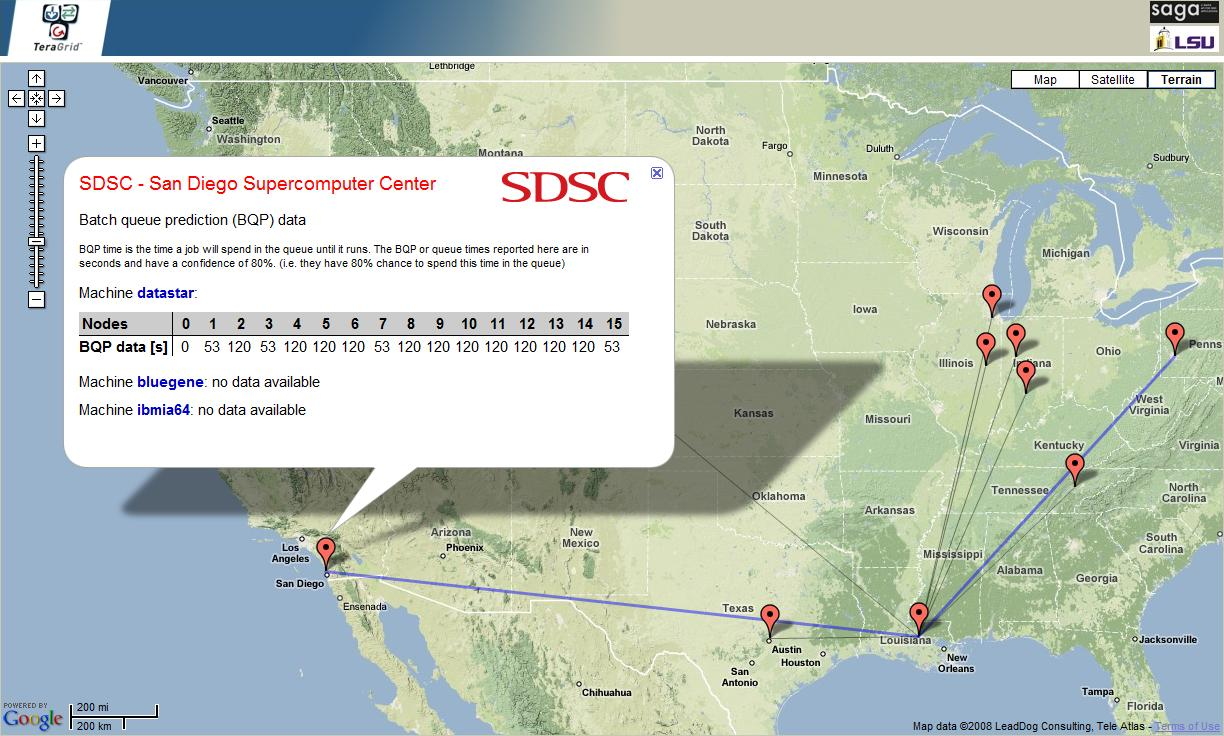
\includegraphics[scale=0.33]{gmaps_bqp.jpg}
\end{center}
\caption{A snapshot of an application using batch-queue-prediction system to dynamically determine the 
best resource to spawn a sub-task to; the noteworthy point is that the entire decision process is at the 
application level -- the fact that the applicaiton has to spawn a job of requirements X is mapped to a
reource requirements, BQP is used to determine the resource based upon optimal availablity and then the 
application uses SAGA to spawn and launch the sub-task onto the chose resource. A paper demonstrating
this feature working across the TeraGrid won the Performance Challenge Award at TeraGrid 2008}
\label{}
\end{figure}

Resource Requirements: For Project 3, we require 200000 SUs; this is the more experimental component
of this proposal, where we do not have clear estimates and benchmarking data. However, based upon our experience/publications alluded to in the previous paragraph, each 
"experiment" that we conduct, (ie application that we develop), requires a minimum of 50000 SUs.

\bibliographystyle{unsrt}
\bibliography{jha_loni_alloc_jul01}

\end{document}



